\documentclass[a4paper, 10pt]{article}
\usepackage[utf8x]{inputenc}
\usepackage{graphicx}
\usepackage{mathenv}
\usepackage{geometry}
\usepackage{amsmath}
\usepackage{textcomp}
\usepackage{subfigure}
\usepackage{amssymb}
\usepackage{amsfonts}
\usepackage{graphics}
\usepackage{pstricks,pstricks-add,pst-math,pst-xkey}
\usepackage{multicol}
\usepackage{xcolor}
\usepackage{listings}
\usepackage{units}
\geometry{hmargin = 2.5cm, vmargin = 1.5cm}

\lstset{
  basicstyle=\ttfamily,
  backgroundcolor=\color{gray!10},
  keywordstyle=\color{green!40!black},
  columns=flexible
}

% OPENING
\title{SY19 - TP04\\Séparateurs à Vaste Marge}
\author{Alice Ngwembou - Antoine Hars}

\begin{document}

\maketitle

\section*{Introduction}

Ce TP a pour but d’étudier les Séparateurs à Vaste Marge.
Nous verrons pour cela les différentes fonctions noyau (linéaire, polynomial et gaussien),
ainsi que l’influence de paramètres, tels que la largeur de bande, sur les résultats obtenus.\\
Nous nous pencherons ainsi sur le cas de données non séparables linéairement,
puis sur le cas de données séparables linéairement.\\
Ensuite nous travaillerons sur la résolution d'un problème de classification par support vector machines étudié dans le cours
et pour finir nous nous attacherons à comprendre comment optimiser les paramètres de coût et de largeur de bande afin d'obtenir un modèle performant.

\section*{Exercice 1}

Nous étudions, dans un premier temps, les Séparateurs à Vaste Marge dans le cas linéairement séparable.\\ \\
Nous avons l'ensemble d'apprentissage dans $\mathbb{R}^{2}$ suivant :\\
$x_{1} = (2,0)$ de la classe $C_{1}$,\\
$x_{2} = (0,2)$, $x_{3} = (-2,2)$ et $x_{4} = (-1,3)$ de la classe $C_{2}$.

\subsubsection*{Question 1 : Donner l’équation de l’hyperplan à vaste marge. Dessiner la frontière de décision
correspondante. Vous indiquez quelles exemples sont des vecteurs support.}

De manière intuitive on devine que la frontière de décision serait $x=y$ pour l'ensemble d'apprentissage donné,
avec les vecteurs de support $x_{1}$ et  $x_{2}$.
\begin{figure}[h!]
\centering
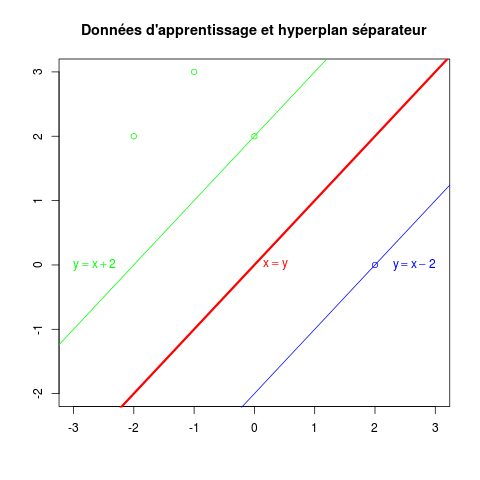
\includegraphics[height = 7cm, width = 7cm]{plots/ex1_hyperplan.png}
\caption{Visualisation de la frontière de décision (en rouge) et de la marge (en vert et en bleu)}
\end{figure}

\newpage
\subsubsection*{Question 2 : Calculer la marge optimale correspondante.}

La marge optimale $\rho$ correspond à la distance la plus courte entre un vecteur et l'hyperplan séparateur.
Les vecteurs (0,2) et (2,0) sont à égale distance de l'hyperplan mais sont aussi les vecteurs les plus proches en distance de l'hyperplan.\\
Il s'agit donc des vecteurs de support, qui sont situés au bord de la marge.\\ \\
La marge optimale $\rho$ équivaut par conséquent à la distance entre $x_{1} = (2,0)$ et son point projeté sur l'hyperplan qui 	a pour coordonnées $(1,1)$.\\
Donc $\rho = \sqrt{2}$.

\subsubsection*{Question 3 : Déterminer la région de R2 pour laquelle une nouvelle observation venant dans l’ensemble
d’apprentissage, et appartenant à $C_{1}$, est sans effet sur la solution (vous donnez l’équation et
vous montrez sur la figure). Idem pour $C_{2}$.}

Une nouvelle observation sera sans effet sur la solution si elle se situe sur ou au dehors de la marge, c'est à dire si elle vérifie :
\begin{figure}[h!]
 \centering
$y >= x + 2$ pour $C_{2}$\\
$y <= x - 2$ pour $C_{1}$
\end{figure}\\
En effet dans le cas contraire, la distance la plus courte d'un vecteur à l'hyperplan serait plus petite.
Par conséquent la marge $\rho$ serait incorrecte et devrait être modifiée. 

\subsubsection*{Question 4 : Donner (en quelques lignes seulement) le code R qui permet d’aboutir à la solution que vous
nommez "model".}

\lstinputlisting[language=R]{sample_code/ex1_model.R}

\subsubsection*{\\Question 5 : Vous expliquez comment on peut confirmer les résultats intuitifs de la première question à
partir du model obtenu (vous montrez les instructions qui permettent de donner les multiplicateurs
de Lagrange et leurs valeurs numériques).}

Dans R on utilise la commande \texttt{model\$SV} pour obtenir les vecteurs de support.
\lstinputlisting[language=R]{sample_code/ex1_vecteursupport.R}
On remarque que les vecteurs de support trouvés de manière intuitive et ceux retournés par R sont les mêmes, ce qui semble confirmer notre intuition.\\ \\
Concernant les multiplicateurs de Lagrange, on utilise la commande \texttt{model\$coefs} qui retourne le produit des coefficients de Lagrange par les facteurs de classe (-1 ou 1).\\
On obtient le résultat suivant :
\lstinputlisting[language=R]{sample_code/ex1_coeflagrange.R}
Comme la valeur 1 est associée au vecteur $(2,0)$ et -1 au vecteur $(0,2)$ alors les valeurs de coefficients de Lagrange sont 0,25 et -0,25.

\newpage
\section*{Exercice 2}

Dans ce deuxième exercice nous étudions la méthode d'optimisation dans le cas non linéairement séparable.

\subsubsection*{Question 1 :}

$\xi$ est porté au carré dans la fonction coût, son signe n’influe donc pas sur l’optimisation de $\frac{1}{2}\sum^{n}_{i=1} \xi^{2}_{i}$

\subsubsection*{Question 2 :}

On ne prend pas en compte les dernières contraintes $\sum^{n}_{i=1}\mu_{i}\xi_{i}$ , ce qui donne :
\begin{figure}[h!]
 \centering
$L(\mathbf{w},w_{0},\xi,\boldsymbol{\alpha},\boldsymbol{\mu}) = \frac{1}{2}| \mathbf{w} |^{2}+\frac{c}{2}\sum^{n}_{i=1} \xi^{2}_{i}-\sum^{n}_{i=1}\alpha_{i}[y_{i}(\mathbf{w'x_{i}}+w_{0})-(1-\xi_{i})]$
\end{figure}

\subsubsection*{Question 3 :}

De l'expression précédente, on obtient les dérivées partielles $ \frac{\partial L}{\partial \mathbf{w}} , \frac{\partial L}{\partial w_{0}}$ et $\frac{\partial L}{\partial \xi_{i}}$ suivantes :
\begin{figure}[h!]
 \centering
$ \frac{\partial L}{\partial \mathbf{w}} =  \mathbf{w} - \sum^{n}_{i=1}\alpha_{i}y_{i}\mathbf{x_{i}}  $\\
$\frac{\partial L}{\partial w_{0}} =  -\sum^{n}_{i=1}\alpha_{i}y_{i}  $\\
$ \frac{\partial L}{\partial \xi_{i}}  =   c\xi_{i} - \alpha_{i}$
\end{figure}\\
Au point selle, ces dérivées sont nulles, par conséquent on obtient :
\begin{figure}[h!]
 \centering
$ \frac{\partial L}{\partial \mathbf{w}} = 0 \Longleftrightarrow \mathbf{w} = \sum^{n}_{i=1}\alpha_{i}y_{i}\mathbf{x_{i}}  $\\
$\frac{\partial L}{\partial w_{0}} = 0 \Longleftrightarrow  \sum^{n}_{i=1}\alpha_{i}y_{i} = 0  $\\
$ \frac{\partial L}{\partial \xi_{i}}  = 0  \Longleftrightarrow  \xi_{i} = \frac{\alpha_{i}}{c} $
\end{figure}

\subsubsection*{Question 4 :}

Pour obtenir le Lagrangien dual $W(\boldsymbol{\alpha})$ on développe le Lagrangien de la \textbf{question 2} :\\

$L(\mathbf{w},w_{0},\xi,\boldsymbol{\alpha},\boldsymbol{\mu}) = \frac{1}{2}| \mathbf{w} |^{2}+\frac{c}{2}\sum^{n}_{i=1} \xi^{2}_{i}-\sum^{n}_{i=1}\alpha_{i}[y_{i}(\mathbf{w'x_{i}}+w_{0})-(1-\xi_{i})]$\\

$L(\mathbf{w},w_{0},\xi,\boldsymbol{\alpha},\boldsymbol{\mu}) = \frac{1}{2}| \mathbf{w} |^{2}+\frac{c}{2}\sum^{n}_{i=1} \xi^{2}_{i} - \sum^{n}_{i=1}\alpha_{i}y_{i}\mathbf{w'x_{i}}  -\sum^{n}_{i=1}\alpha_{i}y_{i}w_{0} +\sum^{n}_{i=1}\alpha_{i} -\sum^{n}_{i=1}\alpha_{i}\xi_{i}$\\ \\
Or on a $ \xi_{i} = \frac{\alpha_{i}}{c}$ , d'où :\\

$W(\boldsymbol{\alpha}) = 
\frac{1}{2}| \mathbf{w} |^{2}
+\frac{c}{2}\sum^{n}_{i=1} (\frac{\alpha_{i}}{c})^{2}
- \sum^{n}_{i=1}\alpha_{i}y_{i}\mathbf{w'x_{i}}  
-\sum^{n}_{i=1}\alpha_{i}y_{i}w_{0} 
+\sum^{n}_{i=1}\alpha_{i} 
-\sum^{n}_{i=1}\frac{\alpha_{i}^{2}}{c}$\\

$W(\boldsymbol{\alpha}) = 
\frac{1}{2}| \mathbf{w} |^{2}
+\frac{1}{2}\sum^{n}_{i=1} \frac{\alpha_{i}^{2}}{c}
- \sum^{n}_{i=1}\alpha_{i}y_{i}\mathbf{w'x_{i}}  
-\sum^{n}_{i=1}\alpha_{i}y_{i}w_{0} 
+\sum^{n}_{i=1}\alpha_{i} 
-\sum^{n}_{i=1}\frac{\alpha_{i}^{2}}{c}$\\

$W(\boldsymbol{\alpha}) = 
\frac{1}{2}| \mathbf{w} |^{2}
- \sum^{n}_{i=1}\alpha_{i}y_{i}\mathbf{w'x_{i}}  
-\sum^{n}_{i=1}\alpha_{i}y_{i}w_{0} 
+\sum^{n}_{i=1}\alpha_{i} 
-\frac{1}{2}\sum^{n}_{i=1}\frac{\alpha_{i}^{2}}{c}$\\ \\
Or on a $\sum^{n}_{i=1}\alpha_{i}y_{i} = 0 \Longleftrightarrow \sum^{n}_{i=1}\alpha_{i}y_{i}w_{0} = 0$, d'où :\\

$W(\boldsymbol{\alpha}) = \frac{1}{2}| \mathbf{w} |^{2} - \sum^{n}_{i=1}\alpha_{i}y_{i}\mathbf{w'x_{i}} +\sum^{n}_{i=1}\alpha_{i} -\frac{1}{2}\sum^{n}_{i=1}\frac{\alpha_{i}^{2}}{c}$\\ \\
Or on a $\mathbf{w} = \sum^{n}_{i=1}\alpha_{i}y_{i}\mathbf{x_{i}} $ , d'où :\\

$W(\boldsymbol{\alpha}) = 
\frac{1}{2} \sum^{n}_{i=1}\sum^{n}_{j=1}\alpha_{i}\alpha_{j}y_{i}y_{j}\mathbf{x_{i}}\mathbf{x_{j}} 
- \sum^{n}_{i=1}\sum^{n}_{j=1}\alpha_{i}\alpha_{j}y_{i}y_{j}\mathbf{x_{i}}\mathbf{x_{j}} 
+\sum^{n}_{i=1}\alpha_{i} 
-\frac{1}{2}\sum^{n}_{i=1}\frac{\alpha_{i}^{2}}{c}$\\

$W(\boldsymbol{\alpha}) = 
\sum^{n}_{i=1}\alpha_{i} 
- \frac{1}{2} \sum^{n}_{i=1}\sum^{n}_{j=1}\alpha_{i}\alpha_{j}y_{i}y_{j}\mathbf{x_{i}}\mathbf{x_{j}}
-\frac{1}{2}\sum^{n}_{i=1}\frac{\alpha_{i}^{2}}{c}$\\ \\ \\
On trouve donc bien un $W(\boldsymbol{\alpha})$ de la forme 
\begin{figure}[h!]
 \centering
$W(\boldsymbol{\alpha}) = \sum^{n}_{i=1}\alpha_{i} - \frac{1}{2}\sum^{n}_{i,j=1}\alpha_{i}\alpha_{j}[y_{i}y_{j}(\mathbf{x_{i}}.\mathbf{x_{j}})+ \frac{\delta_{ij}}{c}]$\\
où $\delta_{ij} = 1$ si $i=j$\\
et $\delta_{ij} = 0$ si $i\neq j$
\end{figure}\\
qui est un problème d'optimisation quadratique.

\newpage
\subsubsection*{Question 5 :}

Le problème dual consiste à maximiser $W(\boldsymbol{\alpha})$ par rapport à $\boldsymbol{\alpha}$ sous les contraintes suivantes
\begin{figure}[h!]
 \centering
$
    \begin{array}{rlll}

 \alpha_{i}  & \geq & 0, &  i = 1, .. , n\\ 
 \xi_{i}  & = & \frac{\alpha_{i}}{c},  &  i = 1, .. , n\\ 
 \sum^{n}_{i=1}\alpha_{i}y_{i} & = & 0 &
      \end{array}
 $
\end{figure}\\ \\
Soit $\boldsymbol{\alpha^{*}}$ la solution de notre problème. Les conditions de Kuhn et Tucker s'écrivent :\\
\begin{figure}[h!]
 \centering
$
    \begin{array}{rlll}

 \alpha_{i}^{*}[y_{i}(\mathbf{w'^{*}x_{i}}+w_{0}^{*})-(1-\xi_{i}^{*})]  & = & 0, &  i = 1, .. , n\\ 
 \xi_{i}  & = & \frac{\alpha_{i}}{c},  &  i = 1, .. , n
      \end{array}
 $
\end{figure}\\ \\
Étant donné que les vecteurs de support ont un $\alpha_{i}^{*} > 0 $ alors :
\begin{figure}[h!]
 \centering
$
    \begin{array}{rlll}
	&\alpha_{i}^{*}& > &0 \\
	\mbox{et} & c & > &0 \\
	\Longleftrightarrow &\frac{\alpha_{i}^{*}}{c} & > & 0 \\ 
	\Longleftrightarrow &\xi_{i}^{*}& > &0
      \end{array}
 $
\end{figure}\\ \\
Par conséquent les vecteurs de support vérifient $\xi_{i}^{*} > 0$.

\subsubsection*{Question 6 :}

On a le Lagrangien dual :
\begin{figure}[h!]
 \centering
$W(\boldsymbol{\alpha}) = \sum^{n}_{i=1}\alpha_{i} - \frac{1}{2}\sum^{n}_{i,j=1}\alpha_{i}\alpha_{j}[y_{i}y_{j}(\mathbf{x_{i}}.\mathbf{x_{j}})+ \frac{\delta_{ij}}{c}]$\\
où $\delta_{ij} = 1$ si $i=j$\\
et $\delta_{ij} = 0$ si $i\neq j$\\
$\Longleftrightarrow W(\boldsymbol{\alpha}) = \sum^{n}_{i=1}\alpha_{i} - \frac{1}{2}\sum^{n}_{i,j=1}\alpha_{i}\alpha_{j}y_{i}y_{j}[(\mathbf{x_{i}}.\mathbf{x_{j}})+ \frac{\delta_{ij}}{cy_{i}y_{j}}]$\\
\end{figure}\\
Or on a $K(\mathbf{x_{i}},\mathbf{x_{j}}) = [(\mathbf{x_{i}}.\mathbf{x_{j}})+ \frac{\delta_{ij}}{cy_{i}y_{j}}]$ tel que :

\begin{figure}[h!]
 \centering
$
    \begin{array}{llrll}
	\mbox{si} & i = j, & \delta_{ij} = 0 & \mbox{donc} & K(\mathbf{x_{i}},\mathbf{x_{j}}) = \mathbf{x_{i}}.\mathbf{x_{j}}\\
	\mbox{si} & i \neq j, & \delta_{ij} = 1 & \mbox{donc} & K(\mathbf{x_{i}},\mathbf{x_{j}}) = \mathbf{x_{i}}.\mathbf{x_{j}} + \frac{1}{c}\\
	 & & \mbox{et } y_{i}y_{j} = 1 & &
      \end{array}
 $
\end{figure}

\newpage
\section*{Exercice 3}

\subsubsection*{Question 1 :}

Le Lagrangien à maximiser par rapport à $\boldsymbol{\alpha}$ est le suivant :
\begin{figure}[h!]
 \centering
$L(\boldsymbol{\alpha})= \sum^{n}_{i=1}\alpha_{i} - \frac{1}{2}\sum^{n}_{i,j=1}\alpha_{i}\alpha_{j}y_{i}y_{j}K(\mathbf{x_{i}},\mathbf{x_{j}})$
\end{figure}\\
avec $K(\mathbf{x_{i}},\mathbf{x_{j}}) = (\mathbf{x_{i}}.\mathbf{x_{j}} + 1)^{2}$ les contraintes
\begin{figure}[h!]
 \centering
$ 0 \leq \alpha_{i} \leq c = 200, i = 1, . ., 5$\\
$\sum^{5}_{i=1}\alpha_{i}y_{i} = 0$
\end{figure}

\subsubsection*{Question 2 :}

On cherche à déduire la valeur $\alpha$ correcte parmi les différents choix proposés :\\ \\
$(a)$ Vu que $\alpha_{i} \geq 0$ pour $i = 1, ..., n$, cette proposition n'est pas la bonne solution car nous avons un $\alpha_{2} = -1$.\\ \\
$(b)$ Nous avons vu que $\sum^{n}_{i=1}\alpha_{i}y_{i} = 0$ mais avec cette proposition, cette somme vaut $1$. Donc la proposition $(b)$ ne convient pas.\\ \\
$(c)$ Cette proposition est la solution que nous validons car nous avons des $\sum^{n}_{i=1}\alpha_{i}y_{i} = 0$ et $0 < \alpha_{i} < \gamma$.\\ \\
$(d)$ Cette proposition ne convient pas malgré le fait qu'elle respecte l'égalité $\sum^{n}_{i=1}\alpha_{i}y_{i} = 0$ car dans ce cas de figure, nous avons $\alpha_{1} > \gamma$ et $\alpha_{4} > \gamma$. $\alpha$ doit respecter : $0 < \alpha_{i} < \gamma$.

\subsubsection*{Question 3}

Afin de vérifier notre hypothèse, nous exécutons le code suivant :\\
\lstinputlisting[language=R]{sample_code/ex3_codeR.R}
La fonction \texttt{svm} est paramétrée avec la fonction noyau polynomiale :
\begin{figure}[h!]
 \centering
$K(\mathbf{x_{i}},\mathbf{x_{j}}) = (\texttt{gamma}*\mathbf{x_{i}}'*\mathbf{x_{i}} + \texttt{coef0})^{\texttt{degree}}$ 
\end{figure}\\
avec \texttt{gamma = 1}, \texttt{coef0 = 1} and \texttt{degree = 2}.

\newpage
\noindent
Les résultats renvoyés par \texttt{model\$SV} correspondent bien à la proposition déduite dans la question précédente, à savoir que $x_{2}$, $x_{3}$ et $x_{5}$ sont des vecteurs propres.\\ \\ \texttt{model\$coefs} nous renvoie les valeurs des coefficients $\alpha_{i}$ des vecteurs propres multipliés par les facteurs de classe (-1 ou 1). Comme $x_{2}$ et $x_{3}$ ont pour facteur 1 et $x_{5}$ a pour facteur -1, on retrouve bien les valeurs de la réponse (c) de la question précédente pour les coefficients de Lagrange des vecteurs propres.

\subsubsection*{Question 4}

Nous avons :
\begin{figure}[h!]
 \centering
$
    \begin{array}{rrllll}
	&\mathbf{K(x_{i},x_{j})} &=& \mathbf{\Phi(x_{i})\Phi(x_{j})} & = & (\mathbf{x_{i}}.\mathbf{x_{j}} + 1)^{2} \\
	\mbox{et} &\mathbf{w} & = &\sum^{5}_{i=1}\alpha_{i}y_{i}\mathbf{\Phi(x_{i})} & &
      \end{array}
 $
\end{figure}\\
La fonction discriminante $g(\mathbf{x}) = \mathbf{w^{*}}.\Phi(\mathbf{x})+w_{0}^{*}$ peut s'écrire sous la forme :

\begin{figure}[h!]
 \centering
$
\begin{array}{rrlll}
& g(\mathbf{x}) &=& \sum_{i \in S}\alpha_{i}y_{i}\mathbf{\Phi(x_{i})}.\mathbf{\Phi(\mathbf{x})}+w_{0}^{*},  &
\mbox{où } S = \{i \in \{1, .. , 5\}, \alpha^{*}_{i} > 0\}\\
\Longleftrightarrow & g(\mathbf{x}) & = & \sum_{i \in S}\alpha_{i}y_{i}\mathbf{K(x_{i},x_{j})} +w_{0}^{*} &\\
\mbox{Alors on a finalement :}  &  &  & &\\
\Longleftrightarrow & g(\mathbf{x}) &= & \sum_{i \in S}\alpha_{i}y_{i}(\mathbf{x_{i}}.\mathbf{x} + 1)^{2} +w_{0}^{*} &
\end{array}
$
\end{figure}

\subsubsection*{Question 5}

On code les fonctions $\mathbf{K(x_{i},x_{j})}$ et $g(\mathbf{x})$ de la manière suivante :
\lstinputlisting[language=R]{sample_code/ex3_codeR2.R}

\newpage
\noindent
On utilise un intervalle de 0 à 7, avec un pas de 0.05 pour le tracé de notre fonction $g(\mathbf{x})$, ce qui nous permet d'afficher la courbe suivante :
\begin{figure}[h!]
\centering
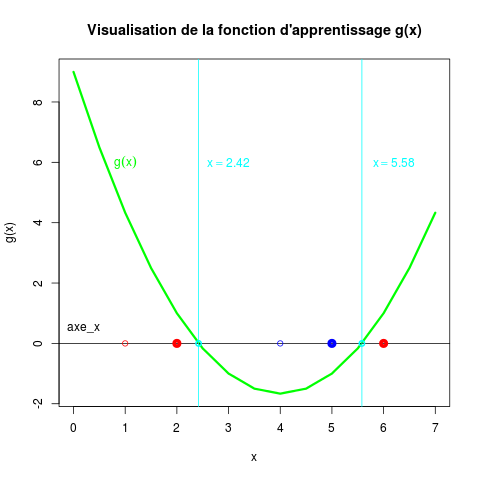
\includegraphics[height = 7cm, width = 7cm]{plots/ex3_graphe.png}
\caption{Visualisation de l'axe des $\mathbf{x}$ avec $\mathbf{x} \in \mathbb{R}$ (en noir), de la fonction discriminante $g(\mathbf{x})$ (en vert), des vecteurs de support $x_{2}$, $x_{3}$ et $x_{5}$  (en gras), des autres vecteurs d'apprentissage (de taille normale) et des classes $C_{1}$ (points rouges) et $C_{2}$ (points bleus).}
\end{figure}\\ \\
Nos données d'apprentissage sont dans l'ensemble à une dimension de $\mathbb{R}$.\\
Par conséquent, on peut les représenter sur la droite des x, chaque vecteur étant un point.\\ \\
Étant donné que l'équation de notre hyperplan correspond à :
\begin{figure}[h!]
\centering
 $g(\mathbf{x}) =  \sum_{i \in S}\alpha_{i}y_{i}(\mathbf{x_{i}}.\mathbf{x} + 1)^{2} +w_{0}^{*}$ = 0, 
\end{figure}\\
les points qui vérifient $g(\mathbf{x}) = 0$ représentent notre hyperplan dans $\mathbb{R}$.\\ \\
Grâce à la fonction \texttt{uniroot} on trouve les deux racines de la fonction $g(\mathbf{x})$ à environ $\mathbf{x} =$ 2.42 et  $\mathbf{x} =$ 5.58 (voir les 2 points en couleur cyan sur la \textit{Figure 2}).\\ \\
La fonction de décision $G(\mathbf{x}) = sgn(g(\mathbf{x}))$ classe les points en $C_{1}$ si  $g(\mathbf{x}) > 0$ et en  $C_{2}$ si  $g(\mathbf{x}) < 0$. Ceci est bien représenté sur notre figure, en effet les vecteurs  $x_{1} = 1$, $x_{2} = 2$ et $x_{3} = 6$ (en rouge) vérifient bien $g(\mathbf{x}) > 0$ et sont donc classés en $C_{1}$ par notre hyperplan, et $x_{4} = 4$, $x_{5} = 5$ (en bleu foncé) vérifient bien $g(\mathbf{x}) < 0$ et sont donc classés en $C_{2}$ par notre hyperplan.\\
Le vecteur $x_{2}$, $x_{3}$ et $x_{5}$ sont les plus proches de l'hyperplan, de plus $x_{2}$ est à la même distance du point $\mathbf{x} =$ 2.42  que les vecteurs $x_{3}$ et $x_{5}$ sont au point $\mathbf{x} =$ 5.58 .\\
Cette distance peut être identifiée comme la marge de l'hyperplan, et notre graphique vérifie donc bien que ces vecteurs sont les vecteurs support de l'hyperplan.

\newpage
\subsection*{Exercice 4 :}

Le but de cet exercice est de mettre en oeuvre la méthode des séparateurs à vaste marge en testant l'influence du choix des paramètres.

\subsubsection*{Question 1 :}

Les fonctions noyau sont de la forme suivante :
\begin{center}
\renewcommand{\arraystretch}{1.8}
\begin{tabular}{|c|c|c|}
\hline
& vu en cours & fonction $svm$ (avec $\gamma = \frac{1}{dimension}$)\\
\hline
\textbf{noyau polynomial} & $\kappa(x,y) = (x'y + 1)^{r}, r > 0$ & $\kappa(x,y) = (\gamma x'y + coef0)^{r}$, $r = 3$ et $coef0 = 0$ par défaut\\
\hline
\textbf{noyau gaussien} & $\kappa(x,y) = exp(-\frac{||x - y||^{2}}{2\sigma^{2}})$ & $\kappa(x,y) = exp(-\gamma |x - y|^{2})$\\
\hline
\end{tabular}
\end{center}
Pour la fonction noyau polynomial, nous pouvons remarquer que $coef0$ dans le cours est mis à $1$ alors que par défaut dans la fonction $svm$, il est à $0$.
$\gamma$ est mis à $1$ dans la fonction du cours alors qu'il est par défaut à $\frac{1}{dimension}$ pour la fonction $svm$.\\ \\
Pour la fonction noyau gaussien, en comparant le cours avec l'expression de la fonction dans $svm$, nous remarquons que $\gamma$ correspond à l'expression $\frac{1}{2\sigma^{2}}$.

\subsubsection*{Question 2:}

Pour cette question, nous travaillons avec le noyau gaussien.\\
\begin{figure}[h!]
\centering
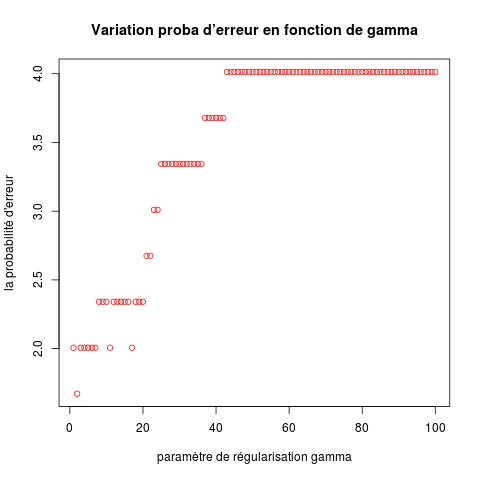
\includegraphics[height = 8cm, width = 8cm]{plots/ex4_q2_proba_erreur_gamma.png}
\end{figure}\\
Sur ce graphique, nous pouvons remarquer que la probabilité d'erreur a tendance à augmenter lorsque le paramètre de pénalisation $\gamma$ augmente.\\
\begin{figure}[h!]
\centering
  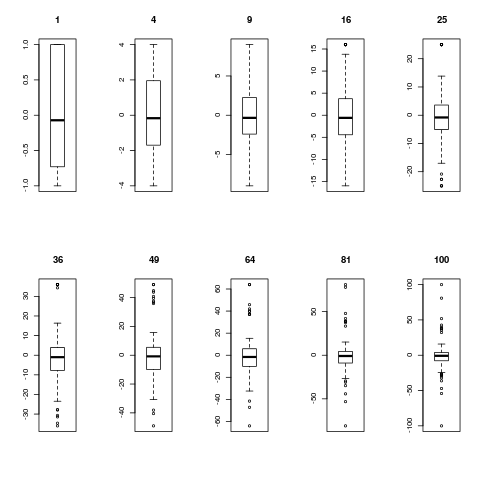
\includegraphics[height = 10cm, width = 15cm]{plots/ex4_q2_boxplot_alpha_.png} 
  \caption{Boxplot sur les composantes du vecteur alpha en fonction du paramètre de pénalisation gamma}
\end{figure}
\newpage
\noindent
Vu que nous avons $0 < \alpha < \gamma$, ce qui nous permet de dire que plus le coût augmente, moins les $\alpha$ sont limités en valeur.\\
Nos graphiques sont cohérents en conclusion car plus $\alpha$ est grand, plus le vecteur de support a de l'importance ou alors ce sera un vecteur aberrant (Le modèle va donc essayer de s'y adapter si le coût est grand, ce qui nous donnera un $\alpha$ élevé.\\ \\
En observant les différents $boxplots$, nous avons remarqué que l'amplitude du vecteur $\alpha$ augmente en fonction de $\gamma$.
Par exemple, nous avons pour un $\gamma = 2$, une amplitude comprise dans l'intervalle $[-2;2]$ et pour un $\gamma = 100$, un $\alpha$ compris dans l'intervalle $[-100; 100]$.\\
Donc nous avons $\alpha$ compris dans l'intervalle $[-\gamma; \gamma]$.\\ \\
Les valeurs d'$\alpha$ peuvent donc atteindre de très grandes valeurs pour un coût élevé, cependant la majorité des alphas restent dans des valeurs "centrales" ou nulles (dans ces cas de figure, le vecteur qui est lié à $\alpha$ n'est pas un support vector).
Le nombre de valeurs extrêmes grandissant, à cause d'un coût augmentant, entraîne une augmentation de la précision de l'hyperplan, voire une trop forte adaptation de celui-ci aux données d'apprentissage quand le coût atteint ses valeurs maximum, ce qui nous donne un modèle très complexe.\\ \\
De plus, nous remarquons, à travers ces graphiques, que pour un paramètre de pénalisation faible, les différentes valeurs de $\alpha$s sont réparties de manière uniforme dans l'intervalle $[-1;1]$.
Alors que plus le paramètre de pénalisation augmente, plus les valeurs d'$\alpha$ semblent avoir tendance à se centrer sur 0 tout en ayant des valeurs aberrantes lorsqu'on dépasse l'intervalle $[-5;5]$ en observant les $boxplots$.\\
Nous pouvons expliquer ce phénomère par la précision grandissante de l'hyperplan.\\ \\
L'endroit où le modèle généralise le plus correspond au moment où il y a le moins d'$\alpha$ positifs, car un $\alpha$ est positif lorsque le vecteur d'apprentissage est un vecteur de support (les vecteurs de support influencent l'hyperplan).\\ \\
Le nombre de vecteurs de support du modèle est important car un nombre trop important implique un modèle très précis qui se généralisera mal, tandis qu’un nombre trop faible implique un modèle peu précis qui sera moins, voire peu efficace.

\newpage
\begin{figure}[h!]
	\centering
  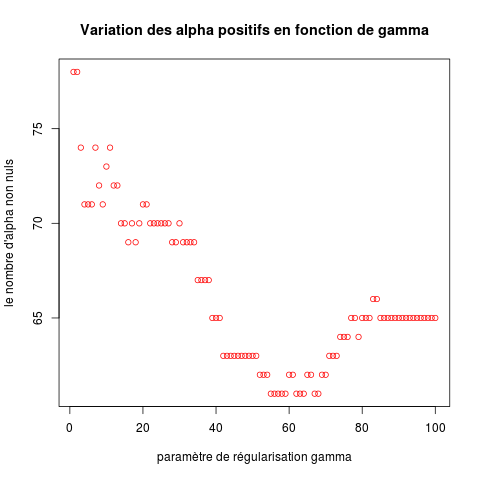
\includegraphics[height = 8cm, width = 8cm]{plots/ex4_q2_alpha_positifs.png}\\
\end{figure}
\noindent
En observant ce graphique, nous pouvons dire que la variation des $\alpha$ positifs ne suit pas les variations de $\gamma$.
Nous obtenons le minimum des $\alpha$ positifs, c'est à dire $\alpha = 61$ pour des valeurs de $\gamma$ proches de 60,
puis les $\alpha$ se stabilisent à 65 pour des $\gamma$ supérieurs à 76.\\
Nous pouvons observer que pour de très faibles valeurs de $\gamma$, la valeur des $\alpha$ est très grande (elle est même à son maximum). Ces valeurs de vecteurs de supports $\alpha$ diminuent progressivement pour des valeurs de $\gamma$ comprises entre 1 et 60 environ.

\subsubsection*{Question 3:}

Nous travaillons dans cette question avec la fonction noyau gaussien.\\
Vu que pour des valeurs de $\gamma$ proches de 100, nous obtenons des valeurs de vecteurs de support $\alpha$ stabilisées,
nous considérons, dans notre cas, que $\gamma = \infty$ peut être assimilé à $\gamma = 100$.
\begin{figure}[h!]
	\centering
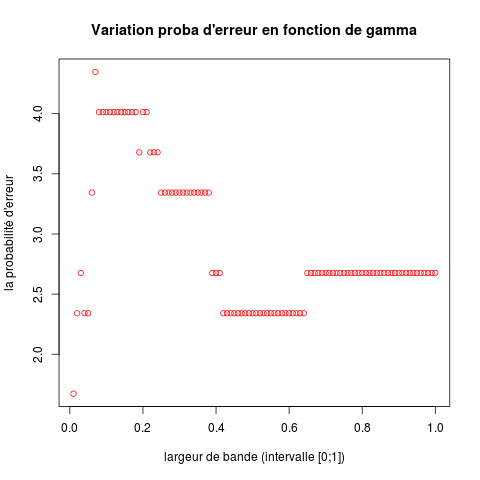
\includegraphics[height = 8cm, width = 8cm]{plots/ex4_q3_proba_erreur_gamma1.png}
\end{figure}\\
Nous pouvons observer sur ce graphique l'évolution des performances de la méthode des Séparateurs à Vaste Marge suivant différentes valeurs de la largeur de bande du noyau gaussien.\\
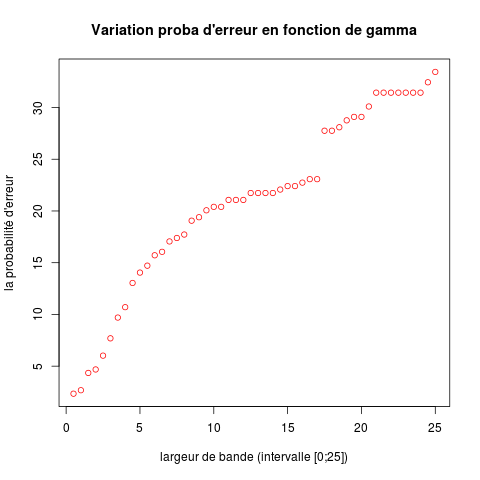
\includegraphics[height = 8cm, width = 8cm]{plots/ex4_q3_proba_erreur_gamma2.png}
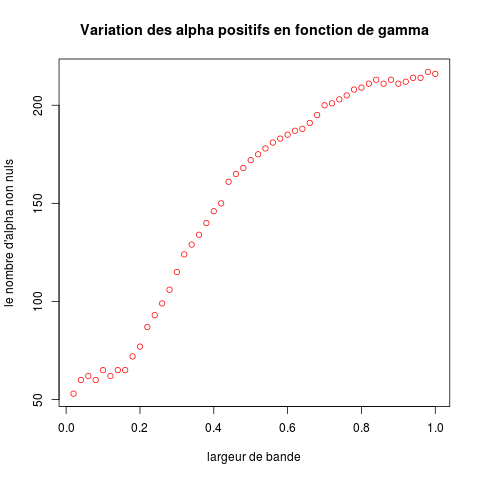
\includegraphics[height = 8cm, width = 8cm]{plots/ex4_q3_alpha_positifs.png}\\ \\
\begin{figure}[h!]
	\centering
  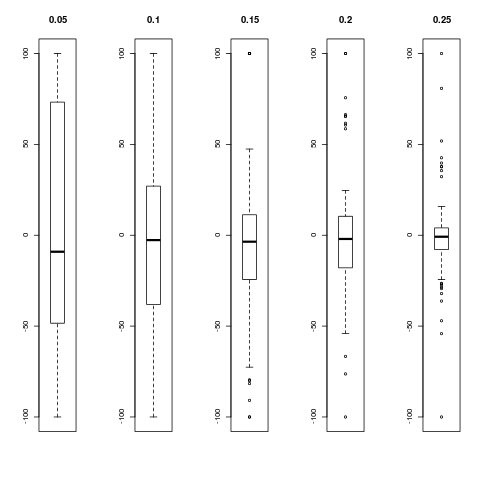
\includegraphics[height = 8cm, width = 10cm]{plots/ex4_q3_boxplot_alpha_.png}
  \caption{Boxplot sur les composantes du vecteur alpha en fonction du paramètre de pénalisation gamma}
\end{figure}\\
Le paramètre $\gamma$ correspond à l’étendue de l’influence de chaque point.
Plus $\gamma$ est faible, plus l’influence est forte; plus $\gamma$ est élevé, plus l’influence est faible.\\ \\
Les valeurs intéressantes se situent pour $\gamma < 1$ car comme nous pouvons l'observer sur le graphique avec une largeur de bande développée sur un intervalle de $[0;25]$, lorsque $\gamma > 1$, le modèle perd rapidement en efficacité.\\
Alors que pour un $\gamma < 1$, la courbe correspondant au pourcentage d’erreur n’est pas linéaire.\\ \\
À l’inverse de ce que l’on a pu observer pour le paramètre de régularisation dans la \textbf{question 2}, le nombre d’$\alpha_{i}$ non nuls varie ici presque linéairement en fonction de la largeur de bande.\\ \\
Pour un $\gamma$ très petit, il y a peu de vecteurs de support et les valeurs des $\alpha_{i}$ sont distribuées uniformément.
Cela signifie que la frontière est lisse et qu'elle n’est pas très précise par rapport aux données d’apprentissage.\\
Lorsque le $\gamma$ augmente, le nombre de vecteurs de support augmente linéairement : l’hyperplan est donc plus précis et adapté à l’ensemble d’apprentissage.\\

\subsubsection*{Question 4:}

\begin{figure}[h!]
	\centering
  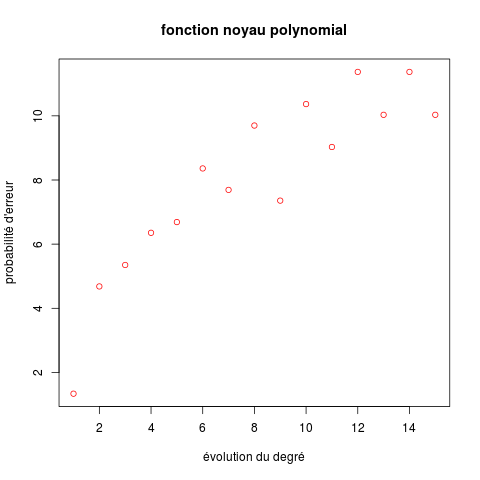
\includegraphics[height = 8cm, width = 8cm]{plots/ex4_q4_polynomial.png}
  \caption{Les probabilités d'erreur sur la fonction noyau polynomiale suivant différentes valeurs de degré.}
\end{figure}
\noindent
Le graphique obtenu montre le pourcentage d’erreur obtenu avec les paramètres optimaux pour le kernel polynomial.\\
Pour ce kernel polynomial, nous avons fait varier le \textit{degré} de 1 à 10, et le meilleur résultat, observé sur le graphique, est obtenu pour un degré égal à 1.\\
Il semble que le kernel polynomial avec un \textit{degré} $= 1$ est efficace.\\ \\
L’autre méthode très efficace est le kernel gaussien étudié tout au
long de ce chapitre, avec un coût égal à 2 (obtenu grâce à la fonction tune()).

\section*{Conclusion}

Pour conclure, tout au long de ce tp, nous avons pu observer l'efficacité des Séparateurs à Vaste Marge dans le cas linéaire et dans le cas non linéaire.\\
Nous avons pu ensuite juger de l'importance des paramètres dans l'utilisation des noyaux polynomial et gaussien pour obtenir un modèle efficace pour résoudre des problème de discrimination en 2 classes. 

\end{document}
